% \documentclass[10pt, a4paper]{amsart}
\documentclass[%
reprint,
nofootinbib,
%superscriptaddress,
%groupedaddress,
%unsortedaddress,
%runinaddress,
%frontmatterverbose,
%preprint,
%showpacs,preprintnumbers,
%nofootinbib,
%nobibnotes,
%bibnotes,
amsmath,amssymb,
aps,
%pra,
%prb,
%rmp,
%prstab,
%prstper,
%floatfix,
]{revtex4-1}
\usepackage[]{graphicx}
\usepackage[]{hyperref}
\usepackage[]{physics}
\usepackage[]{listings}
\usepackage[T1]{fontenc}
\usepackage{color}
\usepackage[]{subcaption}
\usepackage[ruled,vlined]{algorithm2e}

\definecolor{mygreen}{rgb}{0,0.6,0}
\definecolor{mymauve}{rgb}{0.58,0,0.82}

\lstset{ %
  backgroundcolor=\color{white},   % choose the background color; you must add \usepackage{color} or \usepackage{xcolor}
  basicstyle=\footnotesize,        % the size of the fonts that are used for the code
  breakatwhitespace=false,         % sets if automatic breaks should only happen at whitespace
  breaklines=true,                 % sets automatic line breaking
  captionpos=b,                    % sets the caption-position to bottom
  commentstyle=\color{mygreen},    % comment style
  deletekeywords={...},            % if you want to delete keywords from the given language
  escapeinside={\%*}{*)},          % if you want to add LaTeX within your code
  extendedchars=true,              % lets you use non-ASCII characters; for 8-bits encodings only, does not work with UTF-8
  frame=single,	                   % adds a frame around the code
  keepspaces=true,                 % keeps spaces in text, useful for keeping indentation of code (possibly needs columns=flexible)
  keywordstyle=\color{blue},       % keyword style
  language=c++,                    % the language of the code
  otherkeywords={*,...},           % if you want to add more keywords to the set
  rulecolor=\color{black},         % if not set, the frame-color may be changed on line-breaks within not-black text (e.g. comments (green here))
  showspaces=false,                % show spaces everywhere adding particular underscores; it overrides 'showstringspaces'
  showstringspaces=false,          % underline spaces within strings only
  showtabs=false,                  % show tabs within strings adding particular underscores
  stepnumber=2,                    % the step between two line-numbers. If it's 1, each line will be numbered
  stringstyle=\color{mymauve},     % string literal style
  tabsize=2,	                     % sets default tabsize to 2 spaces
}


\begin{document}
	
\title{Eigenvalue Problems: \\
	\normalsize{From Buckling Beam\\
		to Schroedinger's equation in three dimensions} \\
	\hrulefill\small{ FYS3150: Computational Physics }\hrulefill}

\author{Sigurd Sandvoll Sundberg}\homepage{https://github.com/SigurdSundberg/FYS3150/tree/master/project2}

\affiliation{%
	Department of Geosciences, University of Oslo\\
}%

\date{\today}

\begin{abstract}%[0]

\end{abstract}

\maketitle 

\section{Introduction}%[1]
Ordinary differential equation shows up in all parts of physics, with few of them having closed-form solutions, such that approximation schemes are necessary to solve more complicated problems.  These problems are eigenvalue problem to begin, or can be scaled to down to one. Where the physical systems are quite different, but the equations needed to solve them are almost identical. Two seemingly unrelated problems, of a buckling beam and an electron in an harmonic oscillator, when reduced to eigenvalue problems, only have a differing factor of the harmonic oscillator potential. Thus having methods to solve equation on the form 
\begin{equation}
	\mathbf{A} \vec{x} = \lambda \vec{x}
\end{equation}
numerically, is of high relevance. Such methods include Jacobi method, QR factorization, Lanczos' algorithm, bisection method and more. With each method having its own trade off of precision against run time. 

In this study, we will look at two different methods for finding eigenvalues, Jacobi method\cite{GoluVanlJM} and bisection method\cite{barth1967calculation}. The importance of unit tests in code development to make sure algorithms are implemented correctly, especially in large numerical projects, is also discussed alongside its implementations in this project. Secondly, the two eigenvalue problems, buckling beam and one electron in three dimensions are described and discretized, turning them into eigenvalue problems for us to solve. As a benchmark of performance  the Armadillo library and its function $eigsym()$ is used. The mathematical properties and the scaling of Schroedinger's equation is discussed in the appendix. Finally, we discuss our findings and give some concluding remarks.
\section{Algorithms}%[1]
Implementation of the code can be found at: \href{https://github.com/SigurdSundberg/FYS3150/tree/master/project2/code/cpp_codes}{Source Code}
\subsection{Unit tests}%[1]
Unit tests serve a as an easy way of testing code implementation. In large projects, testing all the code at once is not feasible. So rather it is common practice to write unit tests, which ensure that code implementation is done correctly. In addition unit tests help prevent bugs go unnoticed during development this can be critical if multiple people are working on the same project. 
In this study three unit tests have been implemented. The unit tests covers important mathematical properties of the project. 
The tests are as follows;
\begin{itemize}
	\item Setup of Toeplitz matrix - Looking at analytical eigenvalues against computed. 
	\item Finding the largest non-diagonal 
	\item Preservation of eigenvector orthogonality under unitary transformation.
\end{itemize}

\subsection{Jacobi Rotations}\label{jr} %[1]
Jacobi's method for finding eigenvalues and eigenvectors is based on a similarity transformations, that is $A' = S^TAS$. Where $A$ is a real and symmetric matrix of dimensions $A\in \mathbb{R}^{n\times n}$, and the transformation matrix S\footnote{Often referred to as a Givens rotation\cite{stewart2001matrix}, therefore given by $G$ instead of $S$.},  is given by
\begin{equation}
    \label{eqn:givens}
G(i, j, \theta) = 
\begin{bmatrix}
	1 & \dots & 0 & \dots & 0 & \dots & 0 \\
	\vdots & \ddots & \vdots & & \vdots & & \vdots \\
	0 &\dots & \cos\theta & \dots  & - \sin \theta & \dots & 0 \\
	\vdots && \vdots & \ddots & \vdots && \vdots \\
	0 & \dots & \sin \theta & \dots & \cos \theta & \dots & 0 \\
	\vdots && \vdots && \vdots & \ddots & \vdots \\
	0 & \dots & 0 & \dots & 0 & \dots & 1
\end{bmatrix}
\end{equation}
We will refer to the matrix by $S$ from here on. It has the following properties $SS^T = \mathbb{I}$ and $S^T = S^{-1}$, which are easy to check. Our goal is to go from $A$ to a diagonal matrix $D$, which has the eigenvalues of $A$ along its diagonal, in unordered form. This is done by doing multiple similarity transform upon $A$
\begin{equation}
	S_N^T\dots S_1^TAS_1\dots S_N = D
\end{equation}
where $N = 1,2,3,\dots$.
The eigenvectors given by $Ax = \lambda x$, and multiplying by $S^T$ and inserting $S^TS = \mathbb{I}$ we have 
\begin{equation}
	(S^TAS)(S^Tx) = \lambda (S^Tx)
\end{equation}
We recognize $S^TAS$ as $A'$, so it follows that $A'$ has the same eigenvalues as $A$ with the rotated eigenvectors $S^Tx$, the eigenvalues preserve their orthogonality as shown in Appendix \ref{AppA}.

The following notation will be used from now on, $c = \cos\theta$, $s = \sin\theta$ and $t = \tan\theta = s/c$. 
The elements of the matrix $S$ are indexed by $s_{kk} = c = s_{ll}$, $s_{kl} = -s$ and $s_{lk} = s$. The similarity transformation $A' = S^TAS$, we denote the elements of $A$ as $a_{ij}$ and the elements of $A'$ as $b_{ij}$ for all $i,j = 1,2,3,\dots, N$. We then have \cite{mortenJM}
\begin{equation}\label{rotation}
	\begin{split}
		b_{ii} &= a_{ii}, \, i\neq k, i\neq l\\
		b_{ik} &= a_{ik}c - a_{il}s, \, i\neq k, i\neq l\\
		b_{il} &= a_{il}c + a_{ik}s, \, i\neq k, i\neq l\\
		b_{kk} &= a_{kk}c^2 - 2a_{kl}cs + a_{ll} s^2\\
		b_{ll} &= a_{ll}c^2 + 2a_{kl} cs + a_{kk} s^2\\
		b_{kl} &= (a_{kk} - a_{ll})cs + a_{kl}(c^2-s^2)
	\end{split}
\end{equation}
The eigenvectors are found by performing $S^TR$ where $R = \mathbb{I}_N$, its elements are given by $r_{ij}$. The transformed elements are then 
\begin{equation}
	\begin{split}
	r_{ik} &= cr_{ik} - sr_{il}\\
	r_{il} &= cr_{il} + s r_{ik}.
	\end{split}
\end{equation}
In the end the eigenvectors will be row wise in matrix $R$. 

After $N$ similarity transforms we want a diagonal matrix $D$, in other words, we want to set the non-diagonal elements to zero. We require 
\begin{equation}\label{reshuf}
	b_{kl} = b_{lk}=(a_{kk} - a_{ll})cs + a_{kl}(c^2-s^2) = 0 
\end{equation}
Reshuffle \ref{reshuf};
\begin{equation}
	\left(\frac{a_{ll} - a_{kk}}{a_{kl}}\right)cs + c^2-s^2 = 0
\end{equation}
We define 
\begin{equation}
	\tau = \frac{a_{ll} - a_{kk}}{2a_{kl}}
\end{equation}
we obtain the quadratic equation 
\begin{equation}
	t^2 + 2\tau t - 1 = 0
\end{equation}
using $t = s/c$. 

Solving for $t$, we find 
\begin{equation}
	t = -\tau \pm \sqrt{1+\tau^2}
\end{equation}
and we can easily obtain $c$ and $s$ via 
\begin{equation}
	c = \frac{1}{\sqrt{1 + t^2}}
\end{equation}
and $s = tc$. 

The solutions to the quadratic equation is well known, however when $\tau$ becomes large $\sqrt{1 + \tau^2}$ tends to $\tau$. So the entire expression tends to zero. This can be avoided by solve the quadratic equation given by 
\begin{equation}
	1 + \tau\frac{1}{t} - \frac{1}{t^2}= 0
\end{equation}
we find 
\begin{equation}\label{tau}
	t = \frac{1}{-\tau \mp \sqrt{1 + \tau^2}}
\end{equation}
to help with loss of numerical precision. Also we want to choose $\tau$ such that our matrix $A$ tends to a diagonal matrix quickly. This is done by choosing the largest value for expression \ref{tau}. 

In addition to have Jacobi method to converge the fastest, we choose the largest non-diagonal term\cite{GoluVanlJM}. 
We define $M_{ij}$ as the largest non-diagonal element, let $\delta$ be the required tolerance. Also let $R$ be given by $n\times n$ identity matrix.  
The Jacobi algorithm then reads as follows 
\begin{algorithm}[H]\label{algo:JM}
	\SetAlgoLined
	\caption{Jacobi Algorithm}
	initialization\;
	\While{$\abs{M_{ij}^2} \ge \delta$}{
		update $M_{ij}$\;
		find $\tau,c, s, t$\;
		compute the similiarity transform on $A$ and $R$ for $i = k$ and $j = l$\;
	}
\end{algorithm}

Looking at the convergence rate of the Jacobi method, it is typically very poor. On average it needs $3n^2 - 5n^2$ rotations, with each rotations requiring $4n$ floating point operations(FLOPs). Resulting in a total of $12n^3-20n^3$ FLOPs in order to zero out non-diagonal elements\cite{mortenJM}. See a general estimate on the number of iterations(similarity transformations) are needed goes like $O(n^2)$. 

\subsection{Bisection}\label{bi} %[1]
Bisection method is way of root finding, in this case it is used to find the roots of the characteristic polynomial(CP). This implementation is done based on the paper \textit{Calculation of the Eigenvalues of a Symmetric Tridiagonal Matrix by the Method of Bisection}\cite{barth1967calculation}.
\subsubsection{Sturm Sequence}
We are interested in solution to the general polynomial characteristic polynomial found by $det(A - \lambda \mathbb{I})$. It can be shown \cite{datta2010numerical} that the characteristic polynomial can be expressed by 
\begin{equation}\label{ss}
	\begin{split}
		P_0(\lambda) &= 1\\
		P_1(\lambda) &= a_1 - \lambda\\
		P_i(\lambda) &= (a_i-\lambda)P_{i-1}(\lambda) - b_{i-1}^2P_{i-2}(\lambda),\,i = 2,3,\dots,N
	\end{split}
\end{equation}
where $a_{i}$ are the diagonal elements and $b_i$ are the non-diagonal elements defined by $(A - \lambda \mathbb{I})$. This means that $a_{i} = (\text{diagonal element} - \lambda)$. We define $d_i = P_i(\lambda)$ in the same way as characteristic polynomial is defined. 

We are only interested in the roots of the polynomial, or in other words, we want to look at the number times sign changes\cite{AlbrechtCE09}. We define $q_i = d_i/d_{i-1}$ to be the sequence of the number of sign changes in CP. We can rewrite \ref{ss} as 
\begin{equation}
	\begin{split}
		q_1 &= a_1 \\ 
		q_i &= a_i - \frac{b_{i-1}^2}{q_{i-1}} \quad i = 2,3,\dots,N
	\end{split}
\end{equation}
The number of negative value in $r_i$ is equal to the number of roots up to a the given value $\lambda$. Note that $\lambda$ is not the eigenvalues. 

$P_n(\lambda) = d_n$ can be evaluated in $O(n)$ FLOPs. We define $M(x)$ as the function which returns the number of root up to a value $x$. 
\subsubsection{Bisection Algorithm}
The general bisection method bases it self on root finding. Given an interval $x\in[x_0,x_n]$, for a given polynomial $f(x)$ where $f(x_0)*f(x_n) < 0$, there exist a root in the range of $x$. In it simplicity, choose a point $x_{mid}\in (x_0,x_n)$ and check $f_m = f(x_{mid})$. If $a = f_m * f(x_0) < 0$ then there is a root in the interval $x\in [x_0, x_{mid})$. Similar if  $a>0$ then we have $x\in(x_{mid},x_n]$. 

The problem has no info about absolute upper or lower bounds for the eigenvalues and where the roots appear. The absolute bounds can be described by Gerschorin's theorem\cite{AlbrechtCE09}. 

So to find absolute upper and lower bounds for eigenvalues, $y,z$, respectively, we have that 
\begin{equation}
	\begin{split}
		y &= \min_{1\leq i\leq n} a_i - \abs{b_i} - \abs{b_{i-1}}\\
		z &= \max_{1\leq i\leq n} a_i + \abs{b_i} + \abs{b_{i-1}}
	\end{split}
\end{equation}

Given a matrix $A$ of dimension $N\times N$ with $k\leq n$ eigenvalues. We need to find the roots of the characteristic polynomial of dimension $k$. In the algorithm, $k$ denotes the current number of roots left to find. $n$ goes as $n = 1,2,... N$

Let $\epsilon$ be our tolerance between each iterations, such that $\abs{x_{0} - x_{n}} < \epsilon$ then we are satisfied with the answer. We define $x_0$ to be our current smallest value and $x_{max}$ to be our largest current value, those being $x_0 = y$ and $x_{max} = z$. Have $v$ be the empty vector of length $n$, where we store the found eigenvalue. 

The bisection algorithm then reads 
\begin{algorithm}[H]\label{algo:bi}
	\SetAlgoLined
	\caption{Bisection Algorithm}
	initialization\;
	\For{$k=n:-1:1$}{
		\While{$x_{mid} = \abs{x_{0}-x_{n}}/2 > \epsilon$}{
		\If{$M(x_{mid})<k$}{$x_0 = x_{mid}$
			\Else{$x_{max} = x_{mid}$
			}
		}
	}
	$v_k = \abs{x_0 - x_{mid}}/2$ 
}
\end{algorithm}

The bisection method can be evaluated in $O(n)$\cite{barth1967calculation}. 
\section{Implementation} %[1]
\subsection{Classical mechanics: Buckling Beam} %[1]
The first eigenvalue problem we look at is a classical mechanics problem, a buckling beam. Let $u(x)$ describe the vertical displacement of the beam in the $y$ direction. Then we have the following differential equation(DE) 
\begin{eqnarray}
	\gamma\frac{d^2 u(x)}{dx^2} = -Fu(x),
\end{eqnarray}
where $\gamma$ is a constant defined by properties like the rigidity of the beam. The beam has length $L$, $x\in [0,L]$ and a force $F$ applied at $(L,0)$ on the direction towards the origin. 
We solve this equation with Dirichlet boundary conditions, $u(0) = u(L) = 0$ in other words, the end points of the beam are fixed. 
By defining a dimensionless variable $\rho = x/L$, $\rho \in [0,1]$, our equation becomes 
\begin{equation}
	\frac{d^2u(\rho)}{d\rho^2} = -\frac{FL^2}{\gamma}u(\rho) = -\lambda u(\rho)\label{eq:Buckling Beam Disc}
\end{equation}
where $\lambda = FL^2/\gamma$. Our equation \ref{eq:Buckling Beam Disc} when discretized becomes an eigenvalue problem which can be solved numerically. Expanding the above equation using Taylor series to fourth order, gives us the following expression 
\begin{equation}\label{ddu}
	u''(\rho) = \frac{u(\rho + h)- 2u(\rho) + u(\rho- h)}{h^2} + O(h^2)
\end{equation}
where $h$ is the step. By defining minimum and maximum values for $\rho$, $\rho_{min} = 0$ and $\rho_{max} = 1$, respectively. We have for a given number of grid points $N$, that step length $h$ is defined by
\begin{equation}
	h = \frac{\rho_{max} - \rho_{min}}{N}
\end{equation}
The value of $\rho$ at point $i$ is then 
\begin{equation}
	\rho_i = \rho_0 + ih \quad i = 1,2,\dots , N.
\end{equation}
We can rewrite \ref{eq:Buckling Beam Disc} for $\rho_i$ as 
\begin{equation}\label{BB_disc}
-	\frac{u(\rho_i + h) - 2u(\rho_i) + u(\rho_i - h))}{h^2} = \lambda u(\rho_i)
\end{equation}
or in a more compact way as 
\begin{equation}
	-\frac{u_{i+1} - 2u_i + u_{i-1}}{h^2} = \lambda u_i
\end{equation}

Our differential equation \ref{eq:Buckling Beam Disc} can now be rewritten as a matrix problem on the form $A\mathbf{v} = \lambda \mathbf{v}$. 
Where $A$ is a tridiagonal Toeplitz matrix. 

The general form goes as follows 
\begin{equation}\label{TriToe}
	\begin{bmatrix}
		d_1 & e_1 & 0 & 0 & \dots & 0 & 0\\
		e_1 & d_2 & e_2 & 0 & \dots & 0 & 0 \\
		0 &e_2 & d_3 & e_3 & 0 & \dots & 0\\
		\dots&\dots&\dots&\dots&\dots&\dots&\dots\\
		0 & \dots & \dots & 0 & e_{N-3} & d_{N-2} &e_{N-2}\\
		0 & \dots & \dots & \dots & 0 & e_{N-2} & d_{N-1}
	\end{bmatrix}
	\begin{bmatrix}
		u_1\\
		u_2\\
		\dots\\
		\dots\\
		\dots\\
		u_{N-1}
	\end{bmatrix}
	= \lambda 
	\begin{bmatrix}
		u_1\\
		u_2\\
		\dots\\
		\dots\\
		\dots\\
		u_{N-1}
	\end{bmatrix}
\end{equation}
where the endpoints $u_0$ and $u_N$ are excluded. In our case, $d = 2/h^2$ and $a = -1/h^2$. The eigenvalue problem has analytical eigenpairs\cite{tomLyche}, with eigenvalues given as 
\begin{equation}
	\lambda_j = d + 2a\cos\left(\frac{j\pi}{N}\right), \quad j = 1,2,\dots, N-1.
\end{equation}
The eigenvectors are 
\begin{equation}
	\mathbf{u}_j = \left[\sin\left(\frac{j\pi}{N}\right),\sin\left(\frac{2j\pi}{N}\right),\dots,\sin\left(\frac{(N-1)j\pi}{N}\right)\right]^T
\end{equation}
for $j=1,2,\dots,N-1$.

This matrix will function as a baseline for run time and iterations, when comparing Jacobi rotations \ref{jr} and Bisection \ref{bi} later. 
\subsection{Quantum mechanics: One electron in three dimensions} %[1]
The second eigenvalue problem comes from Schroedinger's equation for one electron. The radial part of Schroediner's equation for one electron is 
\begin{equation}
	-\frac{\hbar^2}{2m}\left(\frac{1}{r^2}\frac{d}{dr}r^2\frac{d}{dr}- \frac{l(l+1)}{r^2}\Psi(r) + V(r)\Psi(r) = E\Psi(r)\right)
\end{equation}
We assume $l=0$ and scale the equation as seen in Appendix \ref{AppB} we have 
\begin{equation}\label{Scaled schro implem}
	-\frac{d^2}{d\rho^2}u(\rho) +\rho^2u(\rho) = \lambda u(\rho)
\end{equation}
This equation has analytical solutions for its eigenvalues with $l= 0$ \cite{Project2}. The four first eigenvalues $\lambda$, as follows $\lambda_0 = 3, \lambda_1 = 7, \lambda_3 = 11, \lambda_4 = 15, \dots$. 

We define minimum and maximum values for $\rho$, $\rho_{min} = 0$ and $\rho_{max} = \infty$, such that the $\rho$ has range $\rho\in [0,\infty)$. As setting any value to infinity on a computer is impossible, $\rho_{max}$ is chosen to different values between $[0,\infty)$, such that we reach a desired precision for our eigenvalues. With a given number of grid points $N$, we define the step length $h$, 
\begin{equation}
	h = \frac{\rho_{max} - \rho_{min}}{N}
\end{equation} 
with $\rho$ at point $i$ given by 
\begin{equation}
	\rho_i = \rho_{min}+ih, \quad i = 1,2,3,\dots,N
\end{equation}

Using the same approach as for \ref{BB_disc} we have 
\begin{equation}
		-\frac{u_{i+1} - 2u_i + u_{i-1}}{h^2} + \rho_i^2u_i= \lambda u_i
\end{equation}
Where $\rho_i^2 = V_i$ is the harmonic oscillator potential. 
We define diagonal matrix elements $d_i = 2/h^2 + V_i$ and non-diagonal matrix elements $e_i = -1/h^2$. 
Schroedinger's equation now becomes 
\begin{equation}
	d_iu_i + e_iu_{i+1} + e_iu_{i-1} = \lambda u_i
\end{equation}

The problem of one electron moving in three dimensions is now simplified down to a matrix equation on the same form as for the Buckling Beam, with different diagonal elements and boundary conditions. The eigenvalue problem we are now looking at is on the same form as for the Buckling Beam, namely \ref{TriToe}. The results in the next section for Schroedinger's equation is found by using Jacobi rotations \ref{jr} to find the eigenvalues. 

\section{Results}%[1]
\subsection{Iterations and run time}%[1]
To compare run time between Jacobi method, Bisection method and our baseline being Armadillos $eigsym()$ \cite{DBLP:journals/corr/abs-1805-03380, Sanderson2016}. We have compared the number of iterations to reach value which satisfies a predetermined tolerance $\epsilon$. For the run time comparison twenty(20) runs for different values of $N$ where completed. This is to reduce the effects of cold starts, and get a better base line for the data. 

Looking at the iteration comparison shown in figure \ref{fig:iter}, we can deduce that for the bisection method that it follows $O(n)$ iterations. For Jacobi method, it follows $O(n^2)$ iterations before it converges. This coincides with the estimated results for the number of iterations we can expect with the different methods. 
\begin{figure}[h]
	\centering
	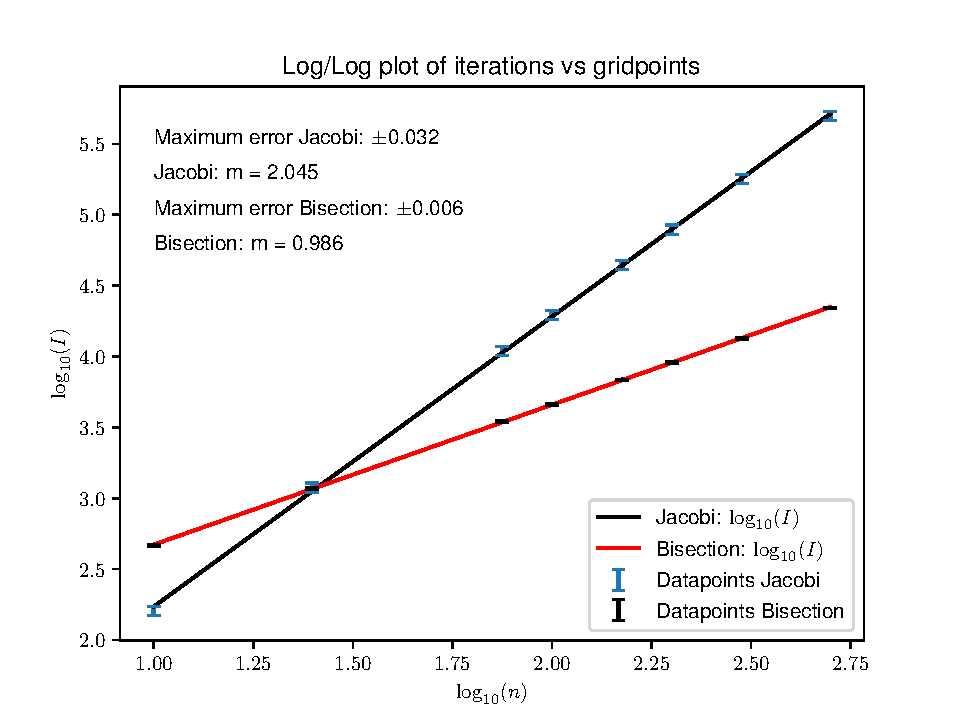
\includegraphics[width=0.47\textwidth]{../code/BB_plot/n_iter.pdf}
	\caption{$\log / \log$ plot of the number of iterations used by algorithm \ref{algo:JM} and \ref{algo:bi}} plotted against the number of grid points $n$. Annotated is the gradient of the linear regression curve and max error between the linear regression and data points. 
	\label{fig:iter}
\end{figure}


We also compared the run time between the three eigensolvers, algo \ref{algo:JM}, algo \ref{algo:bi} and $eigsym()$ from Armadillo. The results from the run time tests are shown in figure \ref{fig:timecomparison}. From the figure we have that for the Jacobi method, has a run time which goes $O(n^{\sim 3.76})$ with $n$. With a fairly stable variation between runs, with a maximum deviation of $\pm 0.12$. 

For the bisection method, it has a run time which goes $O(n^{\sim 1.98})$ or just $O(n^2)$. It in turn has a very low deviation between runs, and its run time extremely stable at a deviation of $\pm 0.02$. 

For the last method, $eigsym()$ which is used as a baseline for testing the algorithms, it has a run time which goes $O(n^{1.75})$. Which is to be expected from a highly optimized linear algebra library, namely Armadillo, and its accompanying libraries LAPACK and BLAS. It has however the largest deviation in run times at $\pm 0.38$. 
\begin{figure}[h]
	\centering
	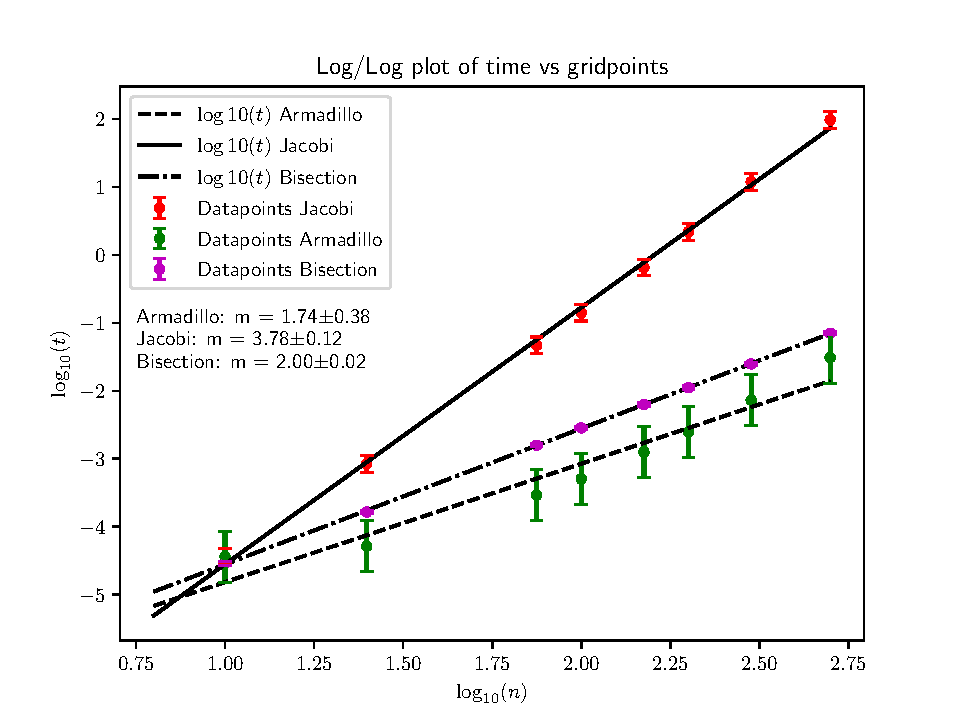
\includegraphics[width=0.47\textwidth]{../code/BB_plot/timecomp.pdf}
	\caption{$\log/\log$ plot of the time used by algorithms \ref{algo:JM}, \ref{algo:bi} and Armadillos $eigsym()$. The gradient of each linear regression curve is shown along side the error bars of the maximum error between the data points and best fit curve. The max error is also shown after the gradient. }
	\label{fig:timecomparison}
\end{figure}

\begin{figure}[h]
	\centering
	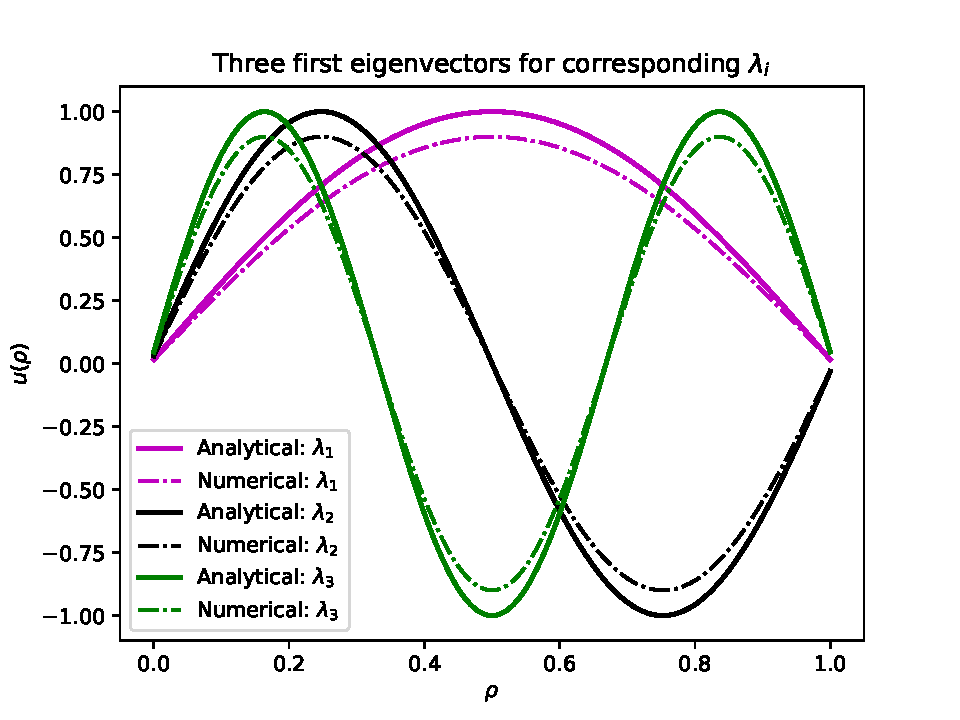
\includegraphics[width=0.47\textwidth]{../code/BB_plot/eigenvec.pdf}
	\caption{The eigenvectors given by $u(\rho)$ for the three first eigenvalues $\lambda_i$ against the analytical counterparts. The numerically found eigenvectors are multiplied by a factor of the relation between the numerical and analytical values times a constant $0.9$ to separate the two graphs. The chosen value for $n$ is 200. It is clear that the two graphs are the same.}
	\label{fig:eigenfunction}
\end{figure}

\subsection{Buckling Beam: Eigenvectors}%[1]
The problem with the buckling beam has known eigenvalues and eigenvectors, thus it is easy to check that an eigenvalue solver is implemented correctly  by comparing the analytical solutions to those found numerically. The analytical and numerically found eigenvectors are shown in figure \ref{fig:eigenfunction}. It is to note that eigenvectors found numerically are scaled to match the analytical eigenvectors by $relation = \frac{v_{analytical}}{v_{numerical}}\times 0.9$. The behavior of eigenvectors is kept under multiplication with a number $c \neq 0$. 

\subsection{Quantum dots}%[1]
We approximated the eigenvalues of one electron in harmonic oscillator with different values for $\rho$ and $n$. The values of $\rho$ used where in the range $[2,10]$ with a step length of $0.2$. For $n$ four different values where used $[100,200,300,400]$. The fairly low resolution is due to lack of computational power and limitations with mainly the Jacobi method, used to find the eigenvalues and eigenvectors. One could choose a higher resolution in either $\rho$ or $n$, but at the lack of time. However when looking at eigenvalues to four significant digits, high resolution of a high value for the estimate of $\rho_{max} = \infty$ is not required. The results are displayed in table \ref{table}. The first four eigenvalues can be approximated by using $\rho_{max} < 6$ and with $n < 500$. 

We can see that all four eigenvalues are estimated to at least $1e-5$ relative precision. Which in our case is within our accepted value for the eigenvalues. Also to note, for the first eigenvalue $n = 200$ was sufficient to reach the wanted precision. 

\begin{table}
	\caption{The table below shows for what value of $\rho$ and $n$ in which we reached a tolerance between the analytical and numerical eigenvalues with an $\epsilon < 10^{-5}$ used for the calculations. To note $n$ was ran for the following value $n=\left\lbrace100, 200, 300, 400\right\rbrace$ and for values of $\rho = 2:0.2:10$.}
	\begin{tabular}{ c|c|c|c|c|c}\label{table}
		$\rho$ & $n$ & Numeric & Analytic & $\abs{\frac{(x_{num} - x_{ana})}{x_{ana}}}$\\ \hline
		3.8 & 200 & 2.999991 & 3 & $3\times 10^{-6}$ \\  
		4.4 & 400 & 7.000046 & 7 & $6.5 \times 10^{-6}$ \\
		4.8 & 400 & 11.00021 & 11 & $1.9 \times 10^{-5}$ \\
		5.2 & 400 & 15.00025 & 15 & $1.6 \times 10^{-5}$
	\end{tabular}
\end{table}


\section{Discussion}%[1]
\subsection{Run time}%[1]
When it comes to run time, the clear looser is the Jacobi method, which is not surprising as it has a slow convergence rate, and is prone to changing elements set to zero, to non-zero values. Such as to repeat already done processes. With the increase in computing power, this algorithm has not aged well, with its main limiting factor being its high run time. It is an easy to implement algorithm, which is both stable and is suited to implementation on parallel processors\cite{mortenJM}. Choosing an $n>1000$ is in most cases not feasible on normal pc, due to the $O(\sim n^4)$ increase in computation time. 

The bisection method performs well, and is also an easy implementation. Its run time of roughly $O(n^2)$ comes from having to loop over $k$ eigenvalues, and root search each polynomial roughly $k$ times. It is also numerically stable in its implementation\cite{barth1967calculation}, dealing with division by zero and negative tolerances. This algorithm can be easily adapted to be used with high and low accuracy by simply changing the wanted tolerance, without risking eigenvalues being inaccurate. It can also be parallelized on a top level. However this algorithm only gives the eigenvalues, so finding the eigenvectors would need to be done in a different implementation. 

For the baseline we have Armadillos eigenvalue solver in $eigsym()$, which performs the fastest as expected by a optimized library. This however had great variation in run time which goes like $O(n^{1.75})$, however from the figure \ref{fig:timecomparison} it is to be noted that for $n=10$($\log_{10}(n) = 1$) that we most likely have an outlier due to low amount of integration points. And that the actual run time of $eigsym()$ is closer to $O(n^2)$. The method chosen by $eigsym()$ to find the eigenvalues are unknown, but can be assumed to be the most efficient methods Armadillo finds after a quick analysis of the given matrix. For a low number of integration points, this could lead to extended run times compared to for larger values of $n$, as a smaller percentage of the run time is used for non-computational time. 
\subsection{Jacobi method: Eigenvectors}%[1]
We have shown in figure \ref{fig:eigenfunction} that our implementation of the Jacobi method, also finds the eigenvalues of our system. The eigenvalues may not be on the form of a traditional eigenvector solver where answer are normally returned in a standardized fashion. 
\subsection{Quantum dots: Eigenvalues}%[1]
We have a trade off between precision, speed and relevance of the data we found. In most cases only the first couple of eigenvalues have any realistic meaning in our world, see buckling beam and figure \ref{fig:eigenfunction} where we would get a system of sine functions with a lower and lower period. Where the higher eigenvectors and values have no real representation. 

The trade off we make here, is mainly between our estimate to $\rho_{max} = \infty$ and the number of grid points we look at. These two are directly related through $\frac{\rho_{max}-\rho_{min}}{n}$ thus leading to a higher estimate for $\rho_{max}$, needing a larger number of grid points $n$. If a large value for $\rho_{max}$ is chosen without an appropriate value for $n$, we have loss of numerical precision, due to lack of integration points. If $n$ is chosen to be too large for the chosen value of $\rho_max$, we can suffer from loss of numerical precision from numbers close to either zero or $\infty$. Including, if the Jacobi method is used we reach a limit around $n = 10000$, where it is no longer possible in a reasonable amount of time to perform the computations without a super computer. Using methods such as the bisection method, can overcome this problem, especially due to the nature of our tridiagonal  Toeplitz matrix\cite{GoluVanlBisection}. 

\section{Conclusion}%[1]
In this project we studied ordinary differential equations and their solutions as eigenvalue problems through the use of the numerical methods. We saw the similarity between a problem from classical mechanics: Buckling beam, and quantum mechanics: Quantum dots with one electron, and how similar to seemingly unrelated problems can become when transformed to an eigenvalue problem. Taking an infinite dimensional problem and through discretization had a finite dimensional problem, that could be solved with the use of linear algebra. 

We implemented two different methods for finding eigenvalues, Jacobi method and bisection method, where only the Jacobi method also gives us the eigenvectors of the problem. The Jacobi method, being an iterative method, we ran it up a a predetermined tolerance for the off-diagonal elements of the matrix close to zero. With the nature of the method, it is prone to set already zeroed out elements to non-zero values, thus increasing the number of iterations needed before the matrix is diagonalized. It was expected that the method would converge in $O(n^2)$ iterations, which coincides with the numerical results. However the method performs very poorly when it comes to time complexity, which goes $O(\sim n^4)$. This makes the algorithm a very poor choice for large $n$. Already for $n= 500$, we see a time usage of $\sim 2$ minutes. If a want for precision, by choosing a large $n$, other more efficient algorithms, especially seen as we have a tridiagonal Toeplitz matrix to begin with is favourable. 
One such algorithm is the bisection method which we also implemented. 

Bisection method has a time complexity of roughly $O(n^2)$, as the characteristic polynomial can be evaluated in $O(n)$ and our need to search for $n$ roots, thus $O(n^2)$. This outperforms the Jacobi method with a factor of $O(n^2)$, which means we can choose large values for $n$ to achieve higher precision. There are upper limits to what values of $n$ that can be chosen, as if $n$ gets too large, one will suffer from loss of precision. 

Looking at our baseline for run time we can conclude that even though the bisection method is more efficient than Jacobi method, there are still improvements that can be made. This is shown by the use of Armadillos $eigsym()$, even though we can approximate its run time to $O(n^2)$, it is safe to assume that Armadillo has a run time for finding eigenvalues for tridiagonal Toeplitz matrices $<O(n^2)$, if not by much, at least slightly. 

Also found is that we can find precise with low amount of integration points, for the three first eigenvectors by use of the Jacobi method, with a relatively low amount of integration points, with $n = 200$, which even though the Jacobi method has a horrible time complexity, it can be used to find eigenvectors with fairly few integration points, for the first couple of eigenvalues. To note is that no tests where done for eigenvectors of higher or lower values of $n$, to compare them to the analytical solutions. However for $n << 200$, we would get a worse approximation of the analytical eigenvectors in the same interval. 

Lastly we looked at the first four eigenvalues for our quantum case. Where we took a continuous problem and approximated it with a finite one. Here we found that $\rho$ can be chosen to a value of at max $5.6$ with $400 \leq n < 500$ and still have good approximations for the first four eigenvalues. As discussed earlier the correlation between $\rho$ and $n$, prevents us from choosing large values of $\rho$, for small values for $n$. This means that if we are interested in later eigenvalues we would need to choose an appropriate $n$, which leads to our Jacobi method being practically unusable. 

The algorithms can be optimized by parallelized computing, even still the Jacobi method has a slow convergence rate. There could be minor improvements to memory in the bisection algorithm, but nothing which would out weight any kind of loss to computation time. For future use, the bisection method is a great implementation if the matrix $A$ in $Ax = \lambda x$ is on the form of a tridiagonal Toeplitz matrix. As there is no need to reduce the matrix to a tridiagonal form, which most other algorithms do, such as Householders\cite{morten}. 

Further one could think of extending the quantum dots with one electron to include multiple electrons.
\appendix %[1]
\section{Preservation of orthogonality and dot product}\label{AppA}%[1]
Consider a basis of vectors $\mathbf{v}_i$, 
\begin{equation}
	\mathbf{v}_i = 
	\begin{bmatrix}
		v_{i1} \\
		\dots\\
		\dots\\
		v_{in}
	\end{bmatrix}
\end{equation}
We assume that the basis is orthogonal, that is 
\begin{equation}
	\mathbf{v}_j^T\mathbf{v}_i = \delta_{ij}
\end{equation}
where $\delta_{ij}$ is the Kronecker-delta.

Let $U$ be a unitary matrix, where $U^{T}U = \mathbb{I}_N$, where $N$ notes the dimension of the identity matrix $\mathbb{I}$.
Let $U$ operate on $\mathbf{v}_i$ such that 
\begin{equation}
	\mathbf{w}_i = U\mathbf{v}_i
\end{equation}
Then 
\begin{equation}
	\mathbf{w}_i^{T}\mathbf{w}_i = \left(U\mathbf{v}_i\right)^{T}U\mathbf{v}_i = \mathbf{v}_i^{T}U^{T}U\mathbf{v}_i = \mathbf{v}_i^{T}\mathbf{v}_i = \delta_{ij}
\end{equation}
 This shows that a unitary transformation of $\mathbf{v}_i$ both preserves the orthogonality and the dot product. $\blacksquare$

\section{Scaling of Schoedinger's equation}\label{AppB}%[1]
In most cases we are not interested in the actual numerical values of physical problems, but rather the behavior of said problems. This makes scaling the equations a central part of natural sciences. 

Given Schroedinger's euqation for one electron
\begin{equation}\label{schro}
	-\frac{\hbar^2}{2m}\left(\frac{1}{r^2}\frac{d}{dr}r^2\frac{d}{dr}- \frac{l(l+1)}{r^2}\Psi(r) + V(r)\Psi(r) = E\Psi(r)\right)
\end{equation}
where we assume spherical symmetry. In our case $V(r)$ is the harmonic oscillator potential $(1/2)kr^2$ with $k=m\omega^2$ and $E$ is the energy of the harmonic oscillator in three dimensions. The oscillator frequency is $\omega$ and the energies are 
\begin{equation}
	E_{nl} = \hbar \omega\left(2n + l + \frac{3}{2}\right)
\end{equation}
with $n = 0,1,2,\dots $ and $l = 0,1,2,\dots$. 
By defining $u(r) = r\Psi(r)$, and substituting into \ref{schro} we obtain 
\begin{equation}
	-\frac{\hbar^2}{2m}\frac{d^2}{dr^2}u(r) + \left(V(r)+\frac{l(l+1)}{r^2}\frac{\hbar^2}{2m}u(r)\right)= Eu(r)
\end{equation}
Since we made a transformation to spherical coordinates we have $r \in [0,\infty)$. We assume $l = 0$. 

Introduce the dimensionless variable $\rho = (1/alpha)r$, which gives $\Psi(\rho) = (1/2)k\alpha^2\rho^2$. Our equation now reads
\begin{equation}
	-\frac{\hbar^2}{2m\alpha^2}\frac{d^2}{d\rho^2}u(\rho) + \frac{k}{2}\alpha^2\rho^2u(\rho) = Eu(\rho)
\end{equation} 
Or equivalently
\begin{equation}
	-\frac{d^2}{d\rho^2}u(\rho) + \frac{mk}{\hbar^2}\alpha^4\rho^2u(\rho) = \frac{2m\alpha^2}{\hbar^2}Eu(\rho)
\end{equation}
By defining $\lambda = \frac{2m\alpha^2}{\hbar^2}E$ and fixing $\alpha = 1$ such that 
\begin{equation}
	\alpha = \left(\frac{\hbar^2}{mk}\right)^{\frac{1}{4}} = 1
\end{equation}
we can rewrite Schroedinger's equation as 
\begin{equation}\label{Scaled Schro}
	-\frac{d^2}{d\rho^2}u(\rho) +\rho^2u(\rho) = \lambda u(\rho)
\end{equation}
%\section{Theory}
%\subsection{The Poisson Equation}
%add section on poisson equation
%>> Dirilect boundary conditions >> relation between f(x) u'' >> Check equal
%\subsection{Approximation of the Second Derivative}
%Add section on approx of second derivative
%>> Going from diff equation >> linear form Av = b >> Matrix -1,2,-1
%\subsection{Relative Error}
%Add short theory of relative error
%>> YES


%%% footnote
% rainforest\footnote{Writing out a general case will also take up more paper
% space}.

%%% Matrix with line through between last elements
% \begin{equation}
% \left[
% \begin{array}{cccc|c}
% 1 & c_1/\beta_1 & 0 & 0 & \tilde{f}_1 \\
% 0 & 1 & c_2/\beta_2 & 0  & \tilde{f}_2 \\
% 0 & 0 & 1 & c_3/\beta_3 & \tilde{f}_3 \\
% 0 & 0 & 0 & 1 & \tilde{f}_4
% \end{array}
% \right] \sim
% \left[
% \begin{array}{cccc|c}
% 1 & c_1/\beta_1 & 0 & 0 & \tilde{f}_1 \\
% 0 & 1 & c_2/\beta_2 & 0  & \tilde{f}_2 \\
% 0 & 0 & 1 & 0 & \tilde{f}_3 -\frac{c_3}{\beta_3}\tilde{f}_4 \\
% 0 & 0 & 0 & 1 & \tilde{f}_4
% \end{array}
% \right]
% \end{equation}

%%% Listing
% \lstinputlisting[language=c++, firstline=146,
% lastline=158]{../problems.cpp}

%%% LU matrix, with diag dots for general case
% \begin{equation}
% A = LU =
% \begin{bmatrix}
% 1 & 0 & 0 & \dots & 0 & 0 \\
% l_{21} & 1 & 0 & \dots & 0 & 0 \\
% l_{31} & l_{32} & 1 & \dots & 0 & 0 \\
%   &\vdots & & \ddots & \vdots  & \\
% l_{n-11} & l_{n-12} & l_{n-13} & \dots & 1 & 0 \\
% l_{n1} & l_{n2} & l_{n3} & \dots & l_{nn-1} & 1
% \end{bmatrix}
% \begin{bmatrix}
% u_{11} & u_{12} & u_{13} & \dots & u_{1n-1} & u_{1n} \\
% 0 & u_{22} & u_{23} & \dots & u_{2n-1} & u_{2n} \\
% 0 & 0 & u_{33} & \dots & u_{3n-1} & u_{3n} \\
%   &\vdots & & \ddots & \vdots  & \\
% 0 & 0 & 0 & \dots & u_{n-1n-1} & u_{n-1n} \\
% 0 & 0 & 0 & \dots & 0 & u_{nn}
% \end{bmatrix}
% \end{equation}

%%% Table
% \begin{table}[h]
% \caption{Elapsed time for increasing $n$}
% \begin{tabular}{lcc}
% \hline
% n & TDMA [s] & LU [s] \\ \hline
% 10 & 0.0000035 & 0.00106083 \\
% 100 & 0.0000116 & 0.0022319 \\
% 1000 & 0.000077892 & 0.0677764 \\
% 10000 & 0.000878769 & 21.9247 \\
% 100000 & 0.00757418 & n/a \\
% 1000000 & 0.08616075 & n/a \\
% 10000000 & 0.76534 & n/a
% \end{tabular}
% \label{tab:solver_times}
% \end{table}

%%% Figure
% \begin{figure}[h]
  % \centering
  % \includegraphics[width=0.9\linewidth]{figures/relerror.png}
  % \caption{Plot of maximum relative error as a function of step size}
  % \label{fig:relerror}
% \end{figure}

%%% Cition and bilbliography%%
% # \emph{Thomas Algorithm} \cite{thomasalgo} How to cite.
% \begin{thebibliography}{10}
  % \bibitem{thomasalgo}{Thomas, L.H. (1949), \emph{Elliptic
        % Problems in Linear Differential Equations over a
        % Network}. Watson Sci. Comput. Lab Report, Columbia University,
      % New York.}
      % \bibitem{morten}{Hjorth-Jensen, M. (2015). \emph{Computational
        % Physics - Lecture Notes 2015}. University of Oslo}
    % \bibitem{golub}{Golub, G.H., van Loan, C.F. (1996). \emph{Matrix
          % Computations} (3rd ed.), Baltimore: John Hopkins.}
% \end{thebibliography}

\bibliography{bib_proj2}
\bibliographystyle{plain}


\end{document}
